\chapter{Regression performance training on a different particle type}\label{app:xtrain_regression}

All the tests so far have assumed that we know exactly what type of particle led to the reconstructed energy deposits.  In a real world situation, the particle identities are not known with complete confidence.  To see how the algorithms above would cope with that situation, we tried training each algorithm on an input sample of electron events, and then we used the trained algorithm to predict the energies for other particle types.

The results are shown in Figure~\ref{fig:reg_nn_cross_gamma} for predicting photon energies and Figure~\ref{fig:reg_nn_cross_pi0} for predicting \pizero\ energies, and are compared to algorithms that are both trained and tested on the same particle type.  In each case, a DNN or CNN trained on electrons is able to achieve the same resolution as a CNN trained on photons or \pizero.  The bias is slightly larger in some cases.

\begin{figure}[hbp]
\centering
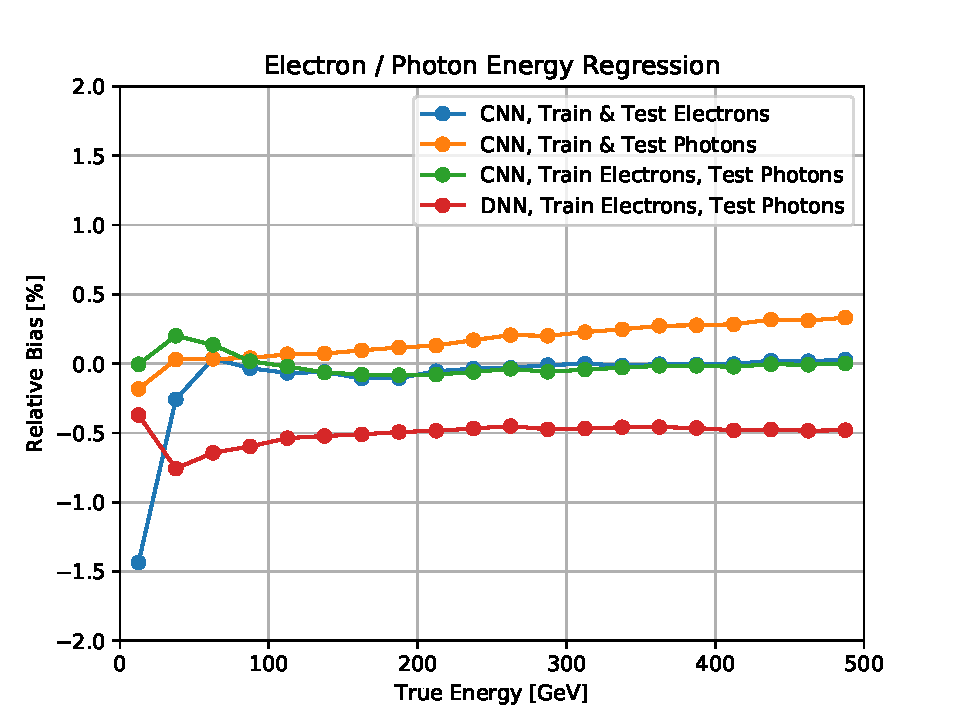
\includegraphics[width=0.38\textwidth]{images/bias_vs_E_EleGammaFixed_nn_cross_zoom.pdf}
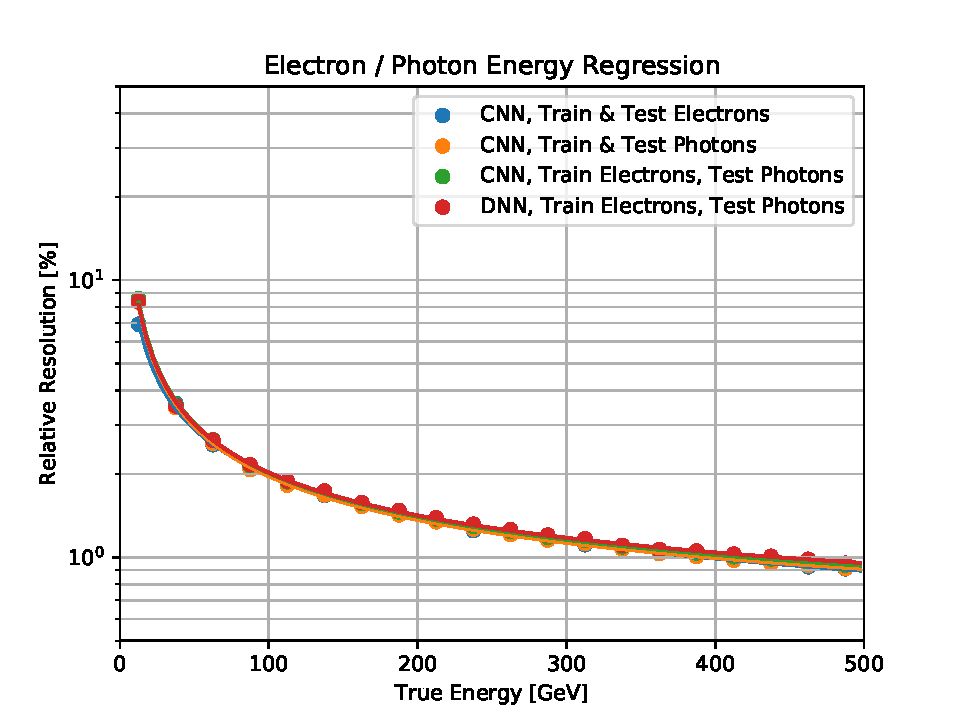
\includegraphics[width=0.38\textwidth]{images/res_vs_E_EleGammaFixed_nn_cross_fits.pdf}
\caption{Bias (top) and resolution (bottom) as a function of true energy, for electrons and photons.  The particles used to train and test each algorithm are given in the legend.
}
\label{fig:reg_nn_cross_gamma}
\end{figure}

\begin{figure}[htbp]
\centering
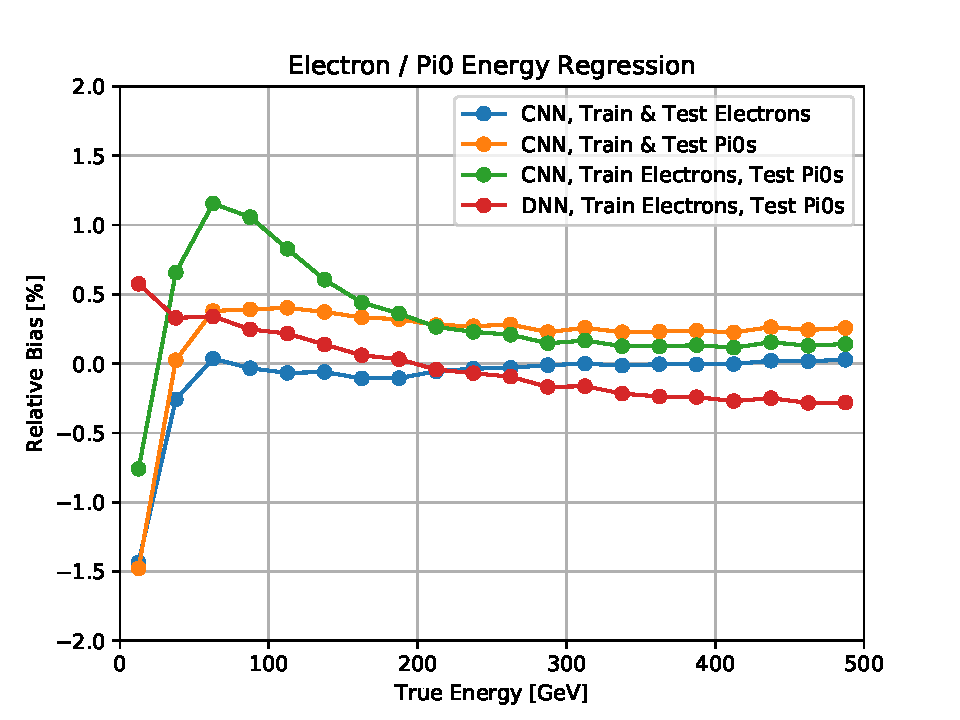
\includegraphics[width=0.38\textwidth]{images/bias_vs_E_ElePi0Fixed_nn_cross_zoom.pdf}
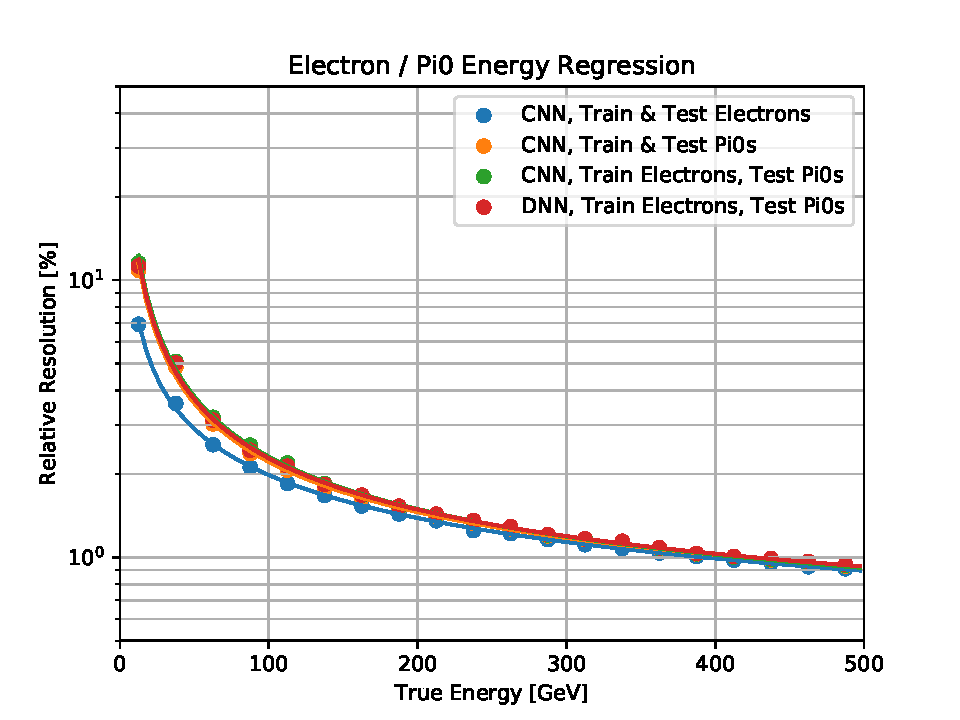
\includegraphics[width=0.38\textwidth]{images/res_vs_E_ElePi0Fixed_nn_cross_fits.pdf}
\caption{Bias (top) and resolution (bottom) as a function of true energy, for electrons and \pizero.  The particles used to train and test each algorithm are given in the legend.
}
\label{fig:reg_nn_cross_pi0}
\end{figure}

Models trained on electrons, photons, or \pizero\ were found to not describe \chpi\ well at all.  This is not surprising given that \chpi\ have a hadronic shower, with a large fraction of energy deposited in the HCAL, compared to the other particles depositing almost all of their energy in the ECAL.

We also checked whether the energy regression was different for photons that have converted into an $e^{+}e^{-}$ pair through interaction with the detector material.  These conversion photons comprise about 9\% of the photon sample.  We tried training and/or evaluating regression models separately on converted photons compared to all photons (which are dominated by unconverted).  The results are shown for XGBoost in Figure~\ref{fig:reg_xgb_conv_gamma} and for CNN/DNN models in Figure~\ref{fig:reg_nn_conv_gamma}.  Worse resolution is seen in each case for converted photons below around 100~GeV, which can be attributed to the subsequent electrons forming two showers instead of one in the calorimeter.  With XGBoost, the resolution remains the same for converted photons when training on the full sample, while for CNN or DNN, the resolution is worse below around 100~GeV.  The bias is also worse for converted photons at lower energy when training on all photons.

\begin{figure}[htbp]
\centering
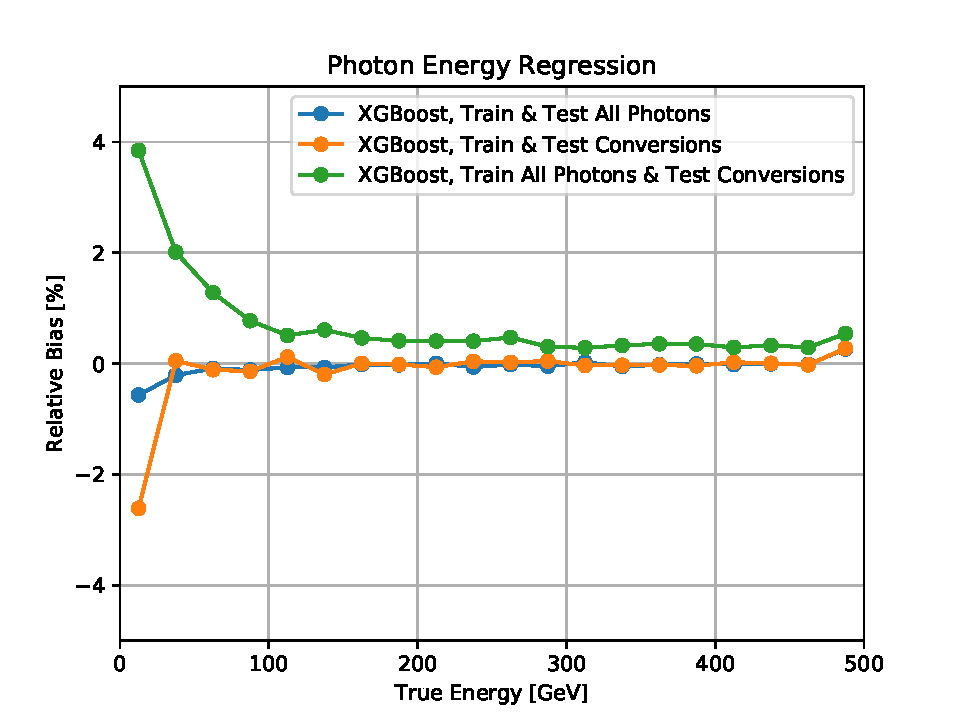
\includegraphics[width=0.38\textwidth]{images/bias_vs_E_GammaFixed_xgb_convs.pdf}
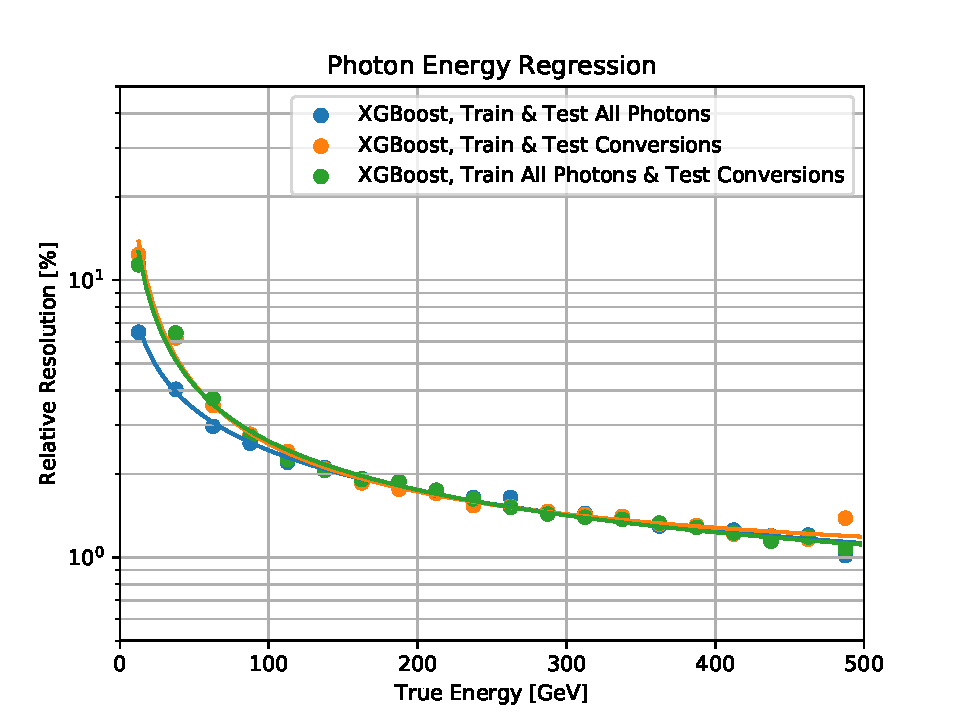
\includegraphics[width=0.38\textwidth]{images/res_vs_E_GammaFixed_xgb_convs_fits.pdf}
\caption{Bias (top) and resolution (bottom) as a function of true energy, for photons using XGBoost regression.  We look at the photon sample when split up by conversions.
}
\label{fig:reg_xgb_conv_gamma}
\end{figure}

\begin{figure}[htbp]
\centering
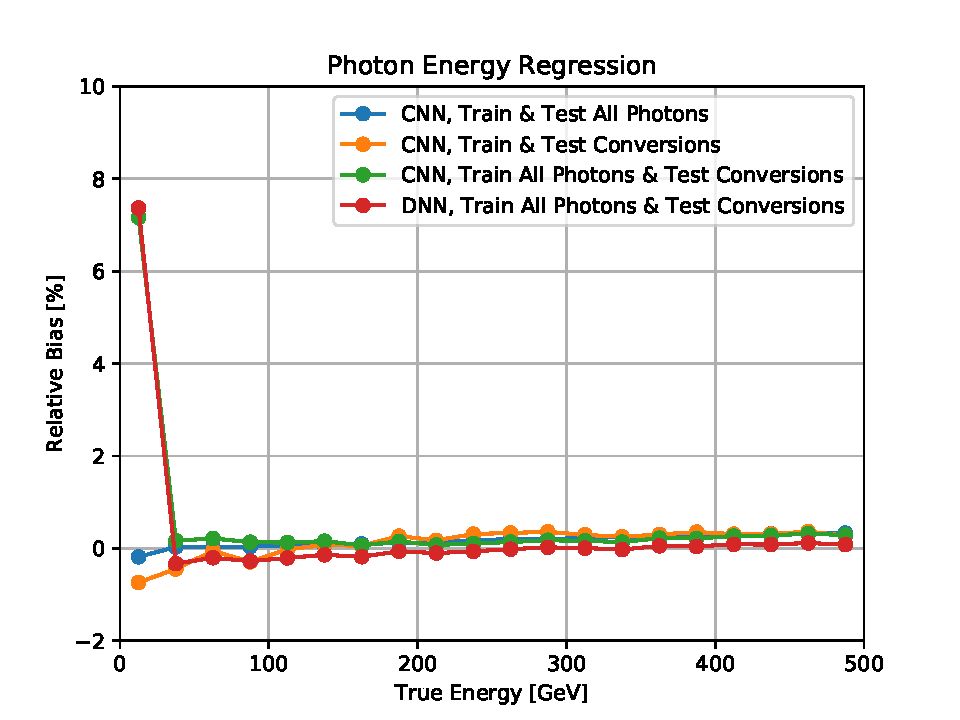
\includegraphics[width=0.38\textwidth]{images/bias_vs_E_GammaFixed_nn_convs.pdf}
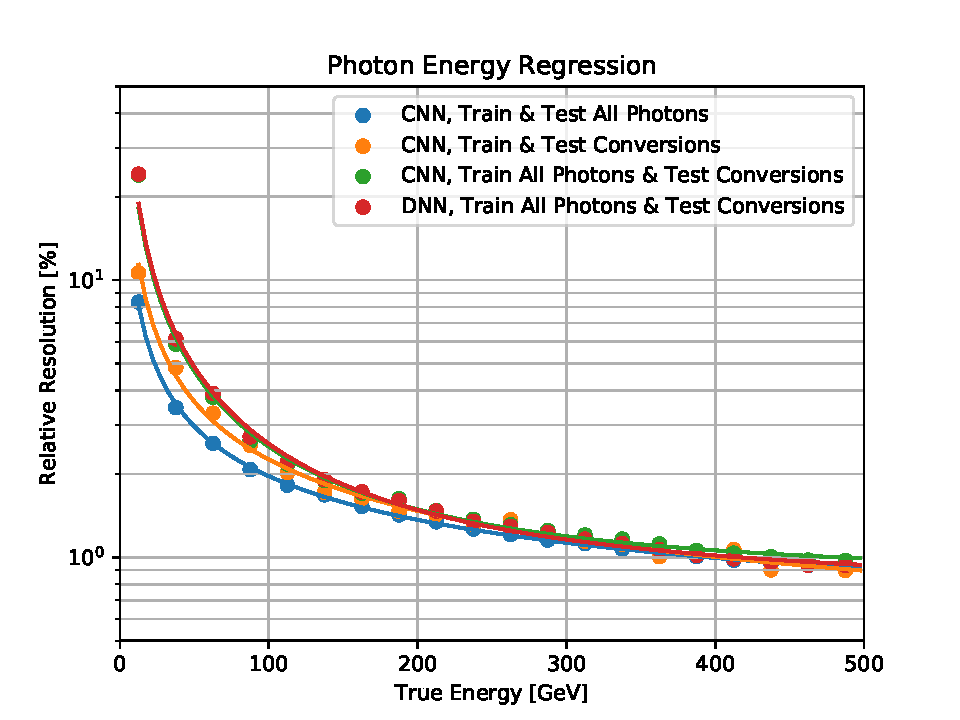
\includegraphics[width=0.38\textwidth]{images/res_vs_E_GammaFixed_nn_convs_fits.pdf}
\caption{Bias (top) and resolution (bottom) as a function of true energy, for photons using CNN or DNN regression.  We look at the photon sample when split up by conversions.
}
\label{fig:reg_nn_conv_gamma}
\end{figure}